\documentclass{article}
\usepackage[utf8]{inputenc}
\usepackage[left=1in,right=1in,top=1in,bottom=1in]{geometry}
\usepackage{authblk}
\usepackage{blindtext}
\usepackage{graphics}
\usepackage{graphicx}
\usepackage{caption}
\usepackage{multirow}
\date{}
\begin{document}
\title{\LARGE \bf
How synthetic data can enhance the performance of machine learning models in the healthcare domain: A murmur detection case study}


\author[1]{Alireza Rafiei\thanks{alireza.rafiei@emory.edu}}

\affil[1]{Department of Computer Science and Informatics, Emory University, Atlanta, GA}

\maketitle

\begin{abstract}
    This is where you write your abstract.
\end{abstract}



\section{Introduction}
The healthcare sector generates and accumulates a vast amount of data every day. This data is critical for medical research, diagnosis, and treatment planning. With the advent of machine learning, this data has become even more valuable for improving patient outcomes and reducing healthcare costs \cite{obermeyer2016predicting}. However, the effectiveness of these cutting-edge technologies is contingent upon the availability and quality of data used for model training \cite{rajkomar2019machine}. In many cases, the datasets available for training machine learning models are insufficient, imbalanced, deficit, and biased, which can hinder progress in harnessing the full potential of machine learning for healthcare \cite{johnson2016machine,dash2019big}. In addition, the sensitive nature of health-related information, along with strict regulatory and security requirements, makes it difficult to obtain and use healthcare data machine learning model development \cite{winter2019governance}. These necessitate the exploration of alternative data generation methods, such as synthetic data, to circumvent these obstacles and propel the field forward.

\par In light of these challenges, synthetic data generation has emerged as a promising avenue for circumventing the limitations associated with real-world healthcare data. By generating new data replicating real-world data's essential characteristics, but with additional variations, synthetic data can facilitate the development of robust and reliable machine learning models in healthcare \cite{chen2021synthetic,murtaza2023synthetic} The adoption of synthetic data in the healthcare domain can also alleviate several pressing concerns, including protecting sensitive patient information and adhering to stringent regulations \cite{gonzales2023synthetic} Additionally, synthetic data generation techniques can contribute to overcoming the challenges posed by the heterogeneous nature of healthcare data since it can be generated in a harmonized format, thereby simplifying the data preprocessing and integration tasks essential for model training. Moreover, synthetic data can help address data quality, completeness, and representation issues by generating balanced and comprehensive datasets that reduce biases and improve the generalizability of machine learning models \cite{das2022conditional}.

\par Heart murmurs, characterized by abnormal heart sounds resulting from turbulent blood flow within the cardiac chambers or through the valves, have garnered significant attention in the medical community due to their potential implications for cardiovascular health. While some murmurs may be benign or physiological, others can indicate underlying pathological conditions that necessitate prompt diagnosis and intervention. The accurate identification and classification of heart murmurs are crucial for guiding clinicians in making informed decisions regarding patient care and management. Physicians typically detect a heart murmur when listening to the heart using a stethoscope or pre-recorded phonocardiography (PCG) of patients. A PCG is a graphical representation of the acoustic signals produced by the heart, displaying the amplitude and frequency of heart sounds and murmurs over time. This technique is particularly useful for detecting, characterizing, and monitoring heart murmurs, as it allows for a more detailed and quantitative assessment of the acoustic properties of these abnormal sounds.

\par In order to develop a dependable machine learning model suitable for real-world applications, a substantial volume of data is necessary \cite{alom2019state}. However, the availability of annotated PCG data specific to certain conditions, such as heart murmurs, remains limited. In addition, the lack of a universally accepted standard for PCG data collection, storage, and analysis further exacerbates inconsistencies and challenges when comparing and integrating data from disparate sources. To overcome these issues, the prospective machine learning model should be trained using a diverse range of data sources. Synthetic PCG data can play a significant role in supplying adequate data to establish a generalizable and robust automated heart murmur detection model.


\par our contribution ....


\section{Materials and methods}
\subsection{The PCG dataset}
The dataset utilized in this study is the CirCor DigiScope PCG dataset \cite{Reyna2022.08.11.22278688,oliveira2021circor}, which is a collection of heart sound signals gathered over two mass screening campaigns in Paraiba, Brazil, from 2014-2015. This dataset was primarily created to study and classify cardiac diseases in a pediatric and pregnant population. Unlike other PCG datasets \cite{clifford2016classification,kazemnejad2021open}, which usually involve a single recording from a single location for each patient, the CirCor dataset includes multiple PCG recordings from various auscultation locations, including pulmonary valve, aortic
valve, mitral valve, and tricuspid valve. Nonetheless, some patients had fewer than four recordings, while a few had multiple recordings from the same location. The recordings were obtained sequentially and may vary in number, location, and duration across patients.

\par The dataset contains 5272 PCG recordings (3163 recordings are publically available) taken from 1568 patients, with an average age of 6.1 (±4.3) years and a range of 0 to 21 years. The PCGs were captured at a sampling rate of 4000 Hz using the DigiScope Collector technology, which is part of the Littmann 3200 stethoscope. The shortest and longest recording durations are 4.8 s and 80.4 s, respectively. The average heart rate is 102 (±20) beats per minute (bpm), with a range of 47 to 193 bpm.

\par The annotations in the dataset provide detailed information about the characteristics of murmurs. They indicate whether a patient has a murmur and present a complete description of the event, including its location, quality, type, shape, pitch, timing, and intensity grade. The expert annotator has also labeled each record as either having a murmur present, absent, or unknown (for low-quality records).


\subsection{Pre-processing}
The PCG recordings were divided into segments of 3 seconds each, using a sliding window technique without overlapping. To represent each segment, a two-dimensional image was created using the logarithmic Mel spectrogram technique. The spectrogram was calculated using the same parameters as in the previous study \cite{elola2022beyond}, including Hamming windows of 25 milliseconds with 50\% overlap and FFT of 512 points in the frequency range 0-800Hz. This frequency range was chosen because murmurs are not typically present in higher frequencies \cite{mcgee2018auscultation}. After applying the Mel filter bank, 32 values were obtained for each frame.
The final representation of every 3-second heard signal recording segment is a 32x240 matrix. The Mel spectrogram depiction of the PCG was opted for this study since it is widely recognized by the audio processing community for its similarity to human hearing. To train the machine learning models, labels were generated for the recording level from the available patient-level label. In this regard, the labels for each recording were assumed to be the same as the patient-level label. The analysis windows for each recording then adopted the label assigned at the recording level.


\begin{figure}
\centering
    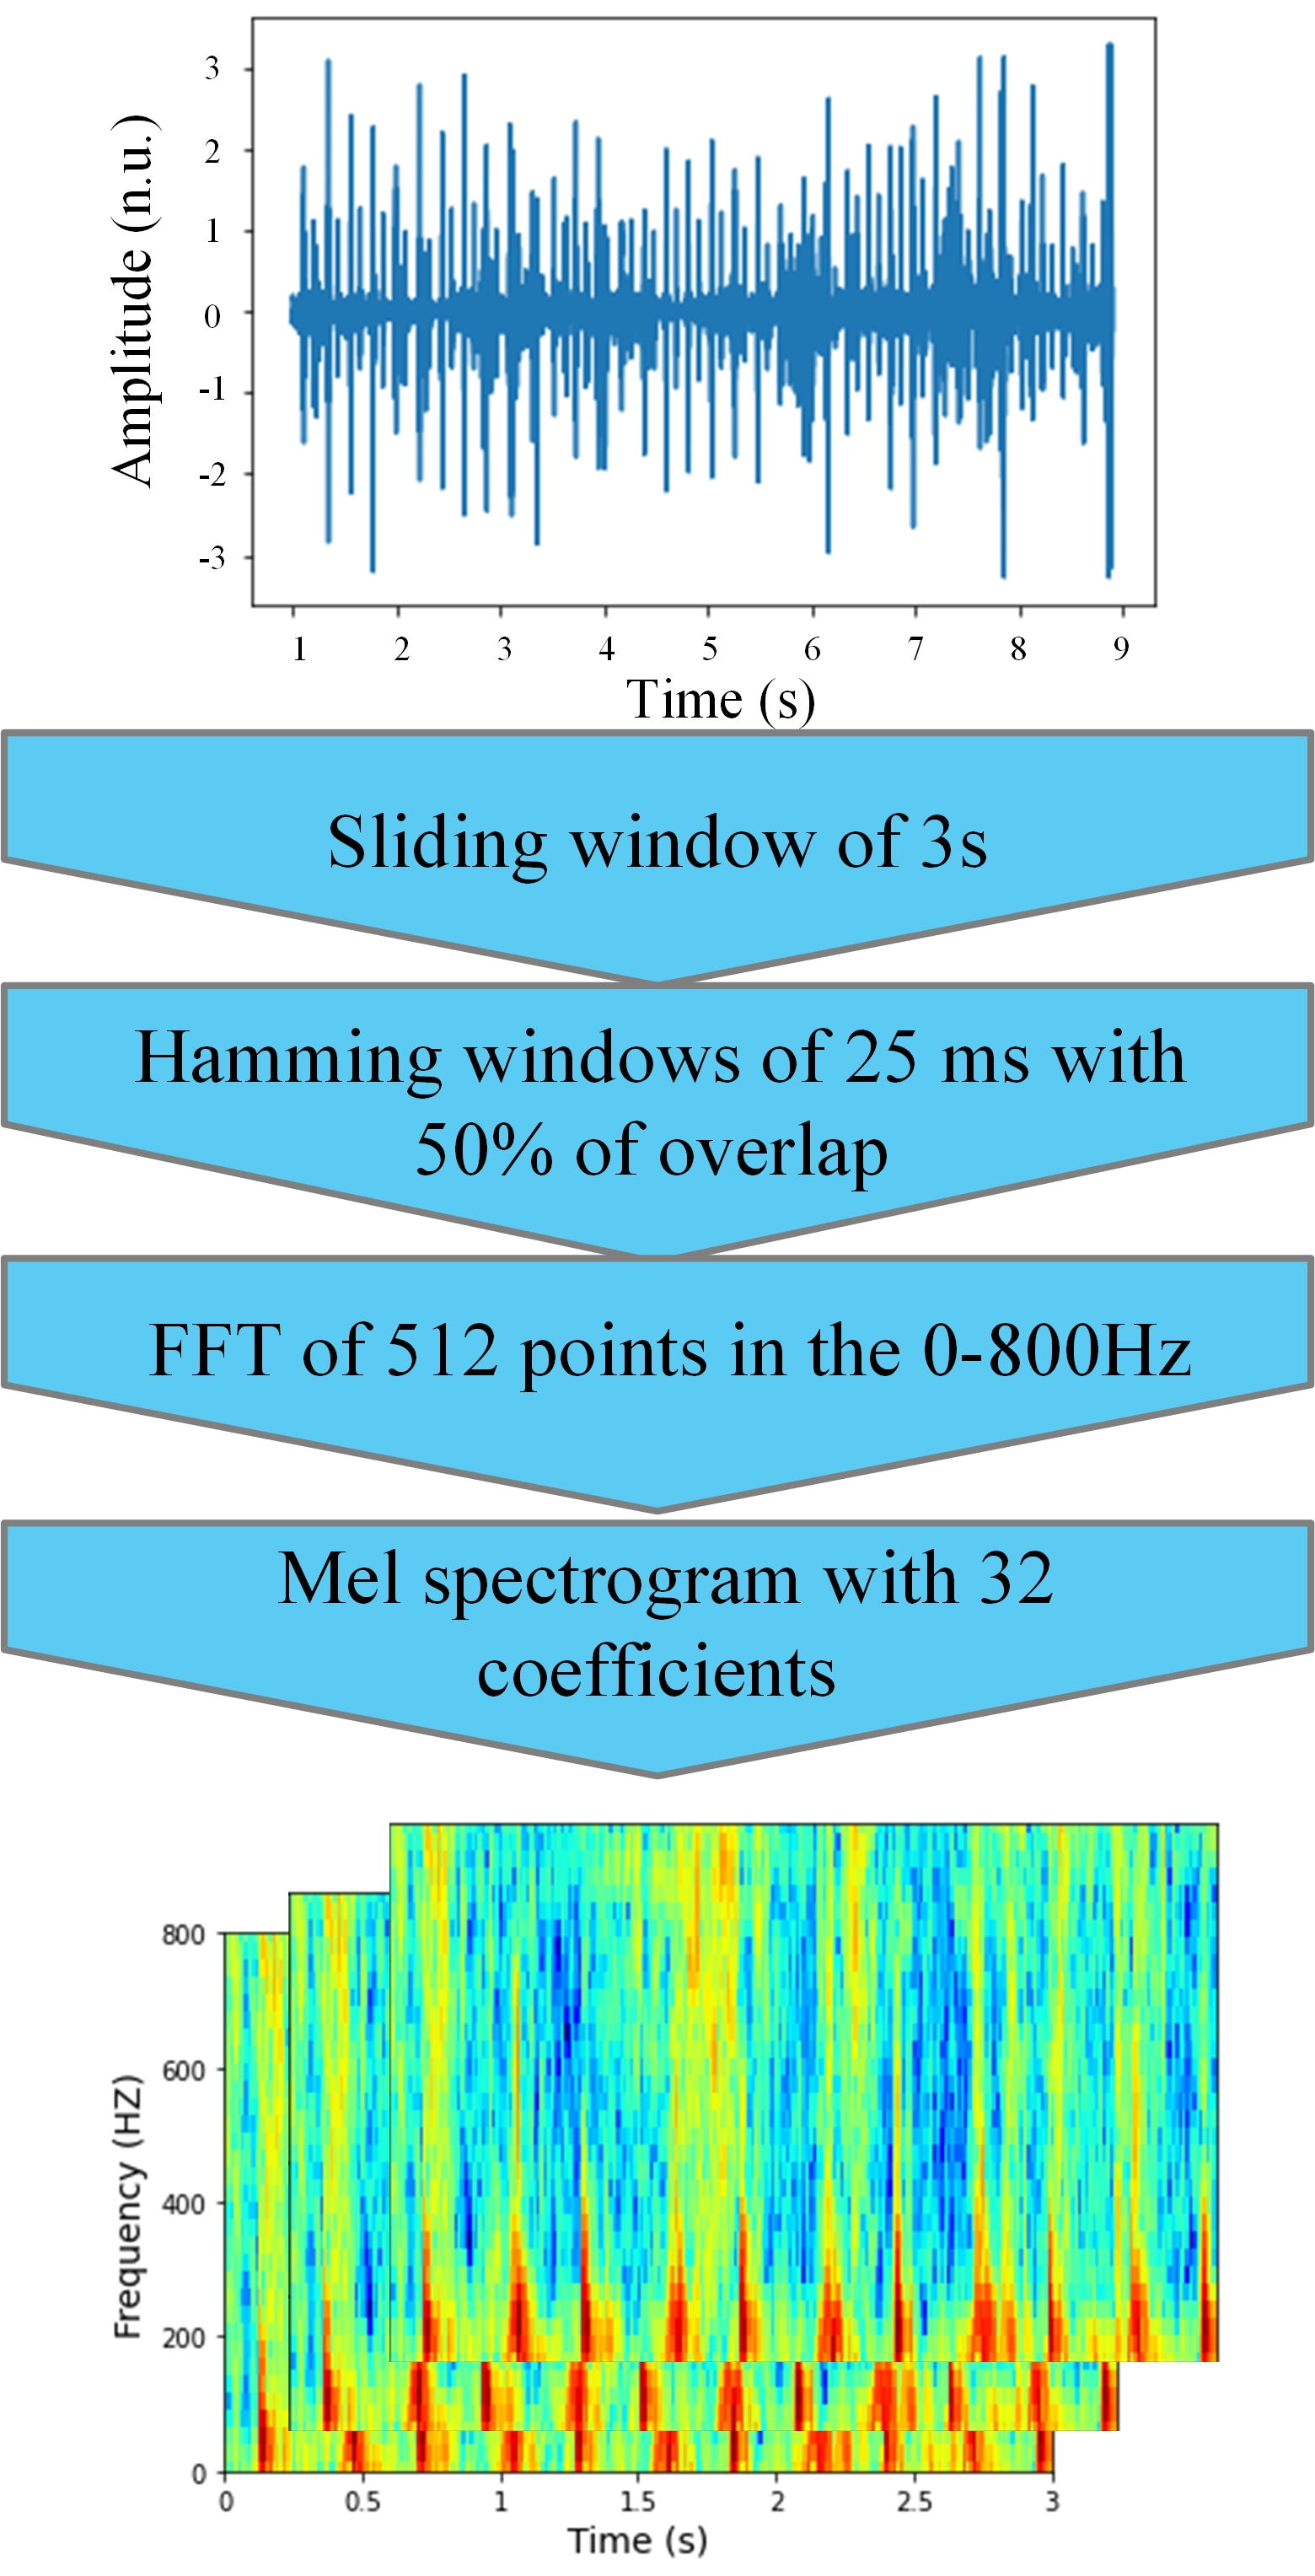
\includegraphics[width=0.4\textwidth]{Documents/preprecessing.jpg}
    \caption{Pre-processing workflow.}
    \label{tab:PP}

\end{figure}


\subsection{Forward modeling}
hospital sound



We calculated the results for the Kullback-Leibler divergence, total variation distance, and Hellinger distance for the two synthetic datasets generated from the original dataset to quantify the dissimilarity between two probability distributions, with lower values indicating a closer resemblance. Upon analyzing the KL divergence values of the two synthetic datasets generated from the original dataset, the amplitude phase altering dataset (0.0957) is more similar to the original dataset than the randomized group delays dataset (0.6685), indicating that the method employed for the amplitude phase altering data generation better preserves the underlying distribution. Similarly, amplitude phase altering dataset (0.0957) has a lower total variation distance compared to the randomized group delays dataset (0.1877), suggesting that this synthetic dataset more closely approximates the original dataset in terms of the probability distribution. The amplitude phase altering dataset also exhibits a smaller Hellinger Distance (0.1010) than the randomized group delays (0.2493), reinforcing that this data is more similar to the original dataset. Across all three measures, synthetic data of the amplitude phase altering technique consistently resembles the original dataset more closely than synthetic data of the randomized group delays approach. This suggests that the first data generation method  is more effective in preserving the original data distribution.

\begin{table}
\centering
\caption{xxx}
\begin{tabular}{|l|l|l|l|}
\hline
Dataset                  & Kullback-Leibler divergence                & Total Variation Distance & Hellinger Distance \\ \hline
Amplitude phase altering & 0.0957                                     & 0.0696                   & 0.1010             \\ \hline
Randomized group delays   & 0.6685  & 0.1877                   & 0.2493  \\ \hline           
\end{tabular}
\end{table}

\begin{figure}
\centering
    \includegraphics[width=1\textwidth]{Documents/Generated data.jpg}
    \caption{xxx.}
    \label{tab:GD}

\end{figure}


\begin{figure}
\centering
    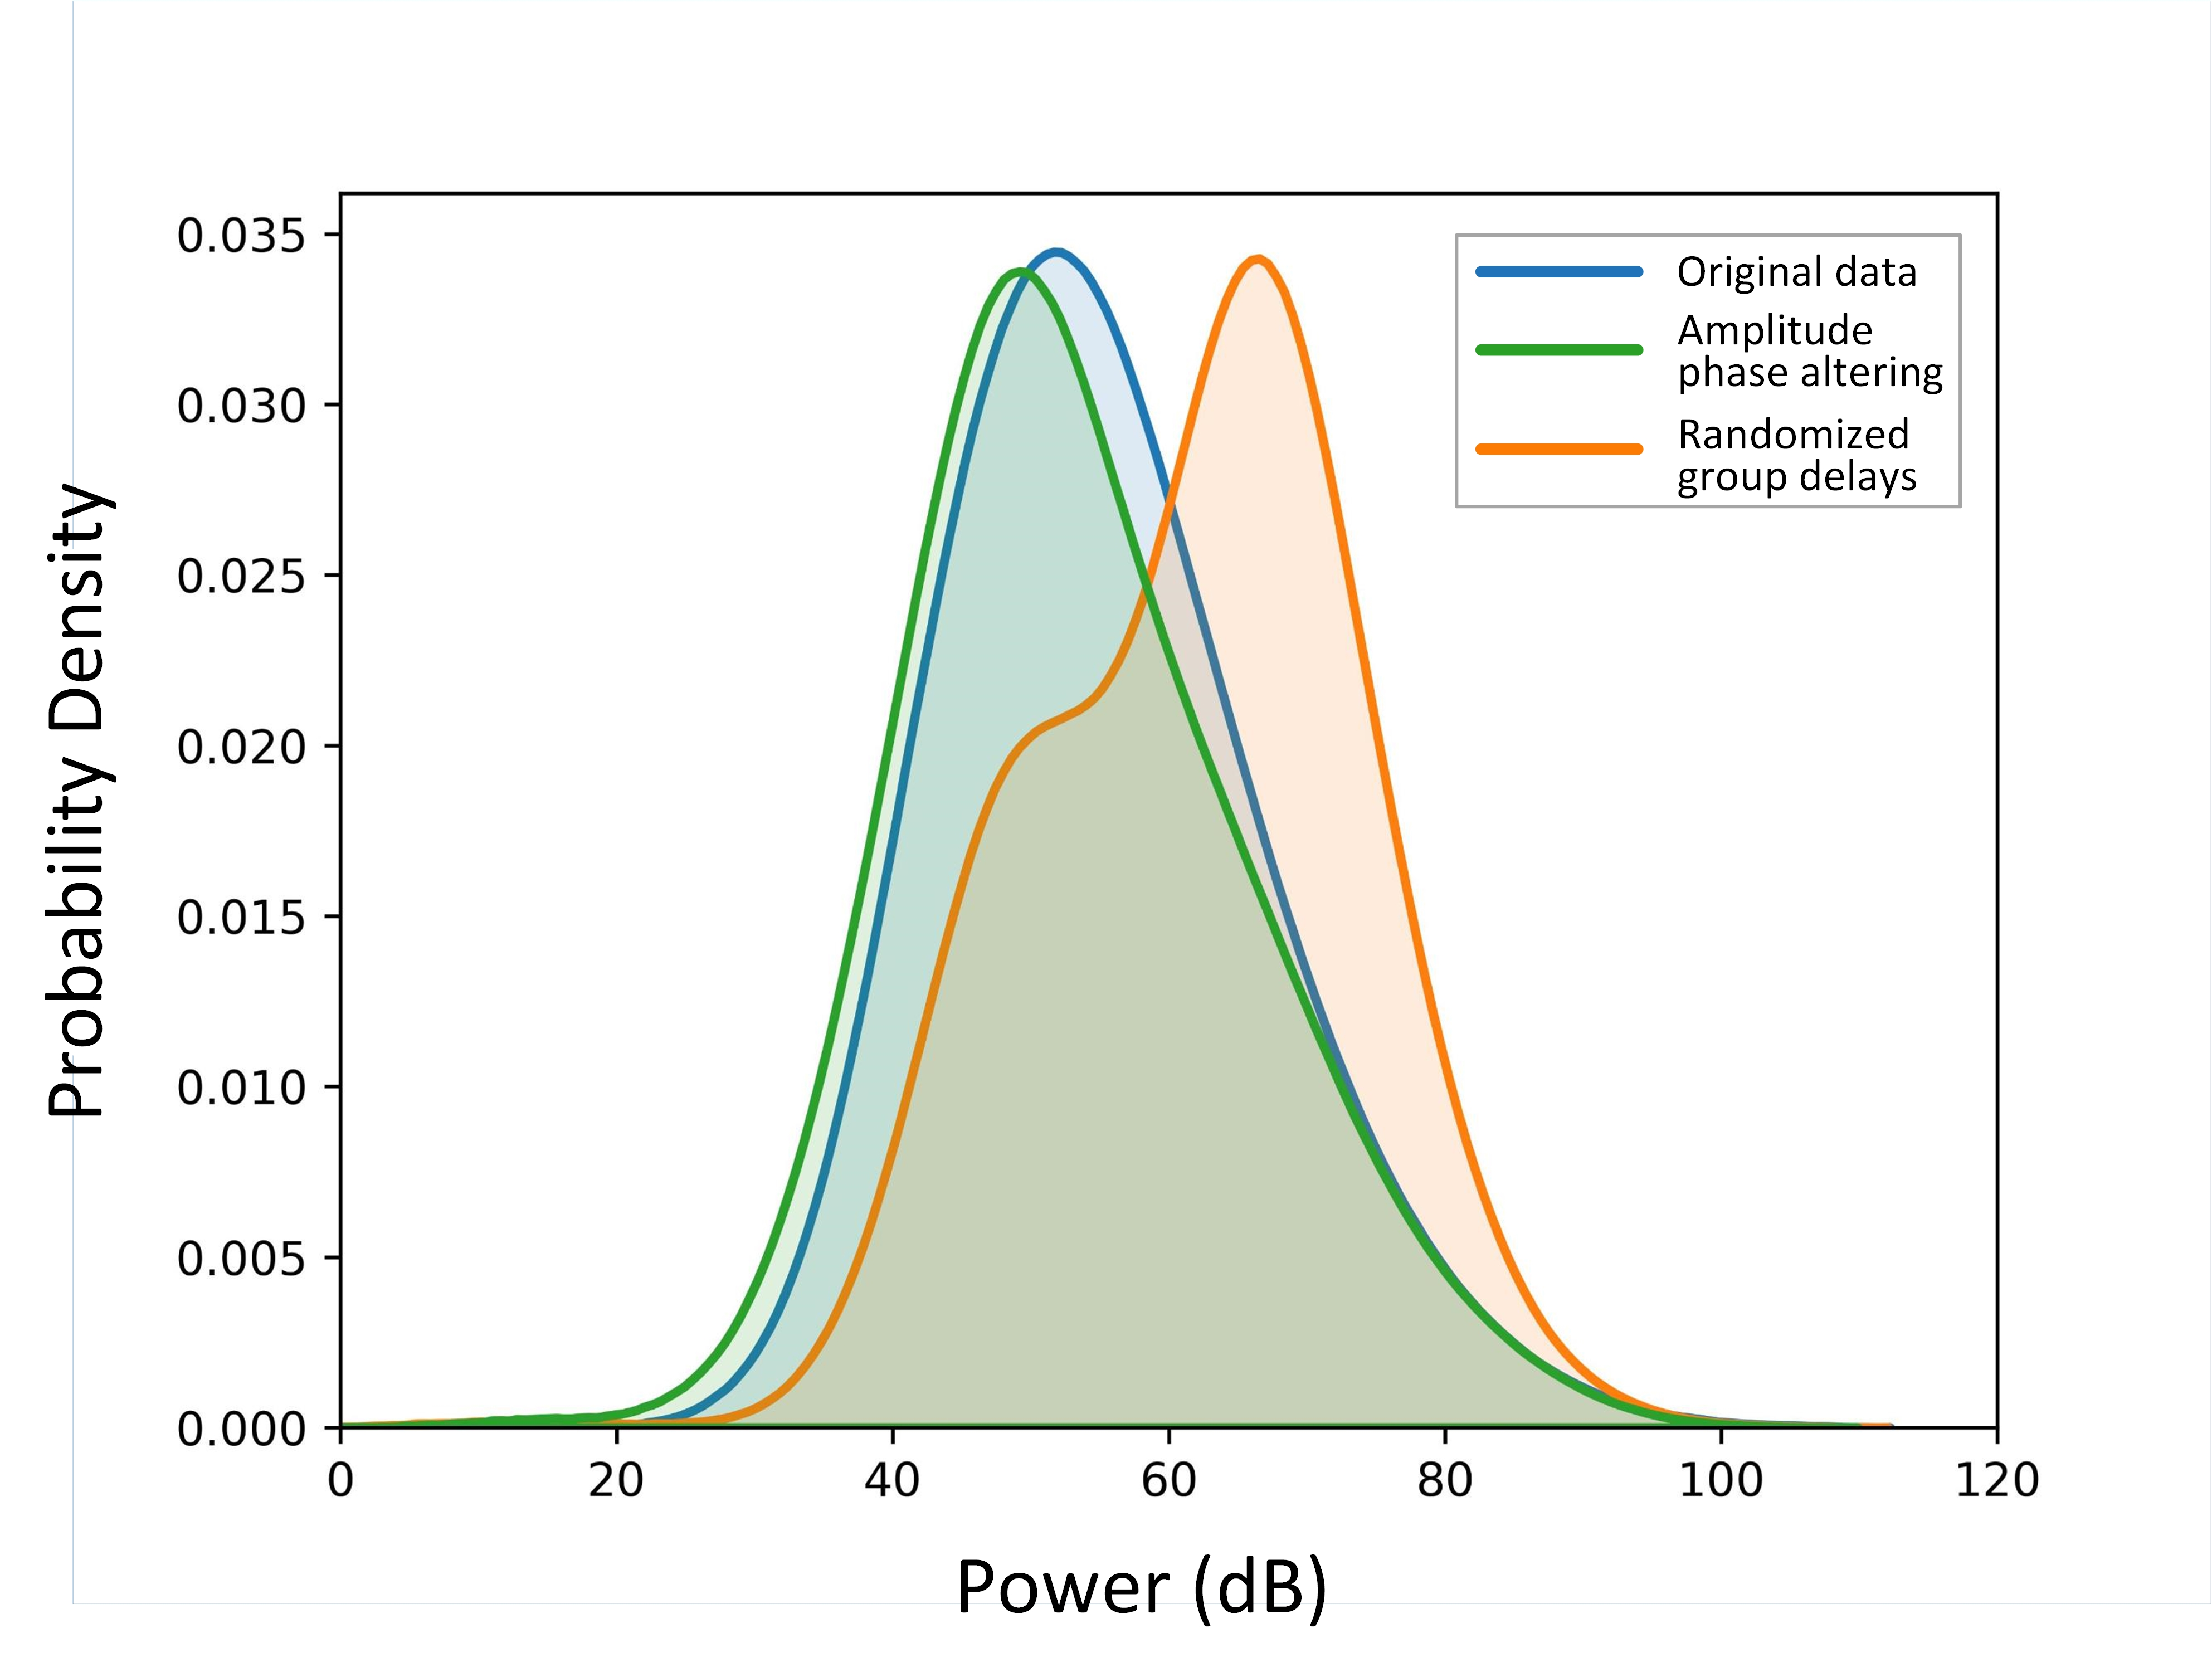
\includegraphics[width=0.6\textwidth]{Documents/pd.jpg}
    \caption{xxx}
    \label{tab:PD}

\end{figure}


\begin{figure}
\centering
    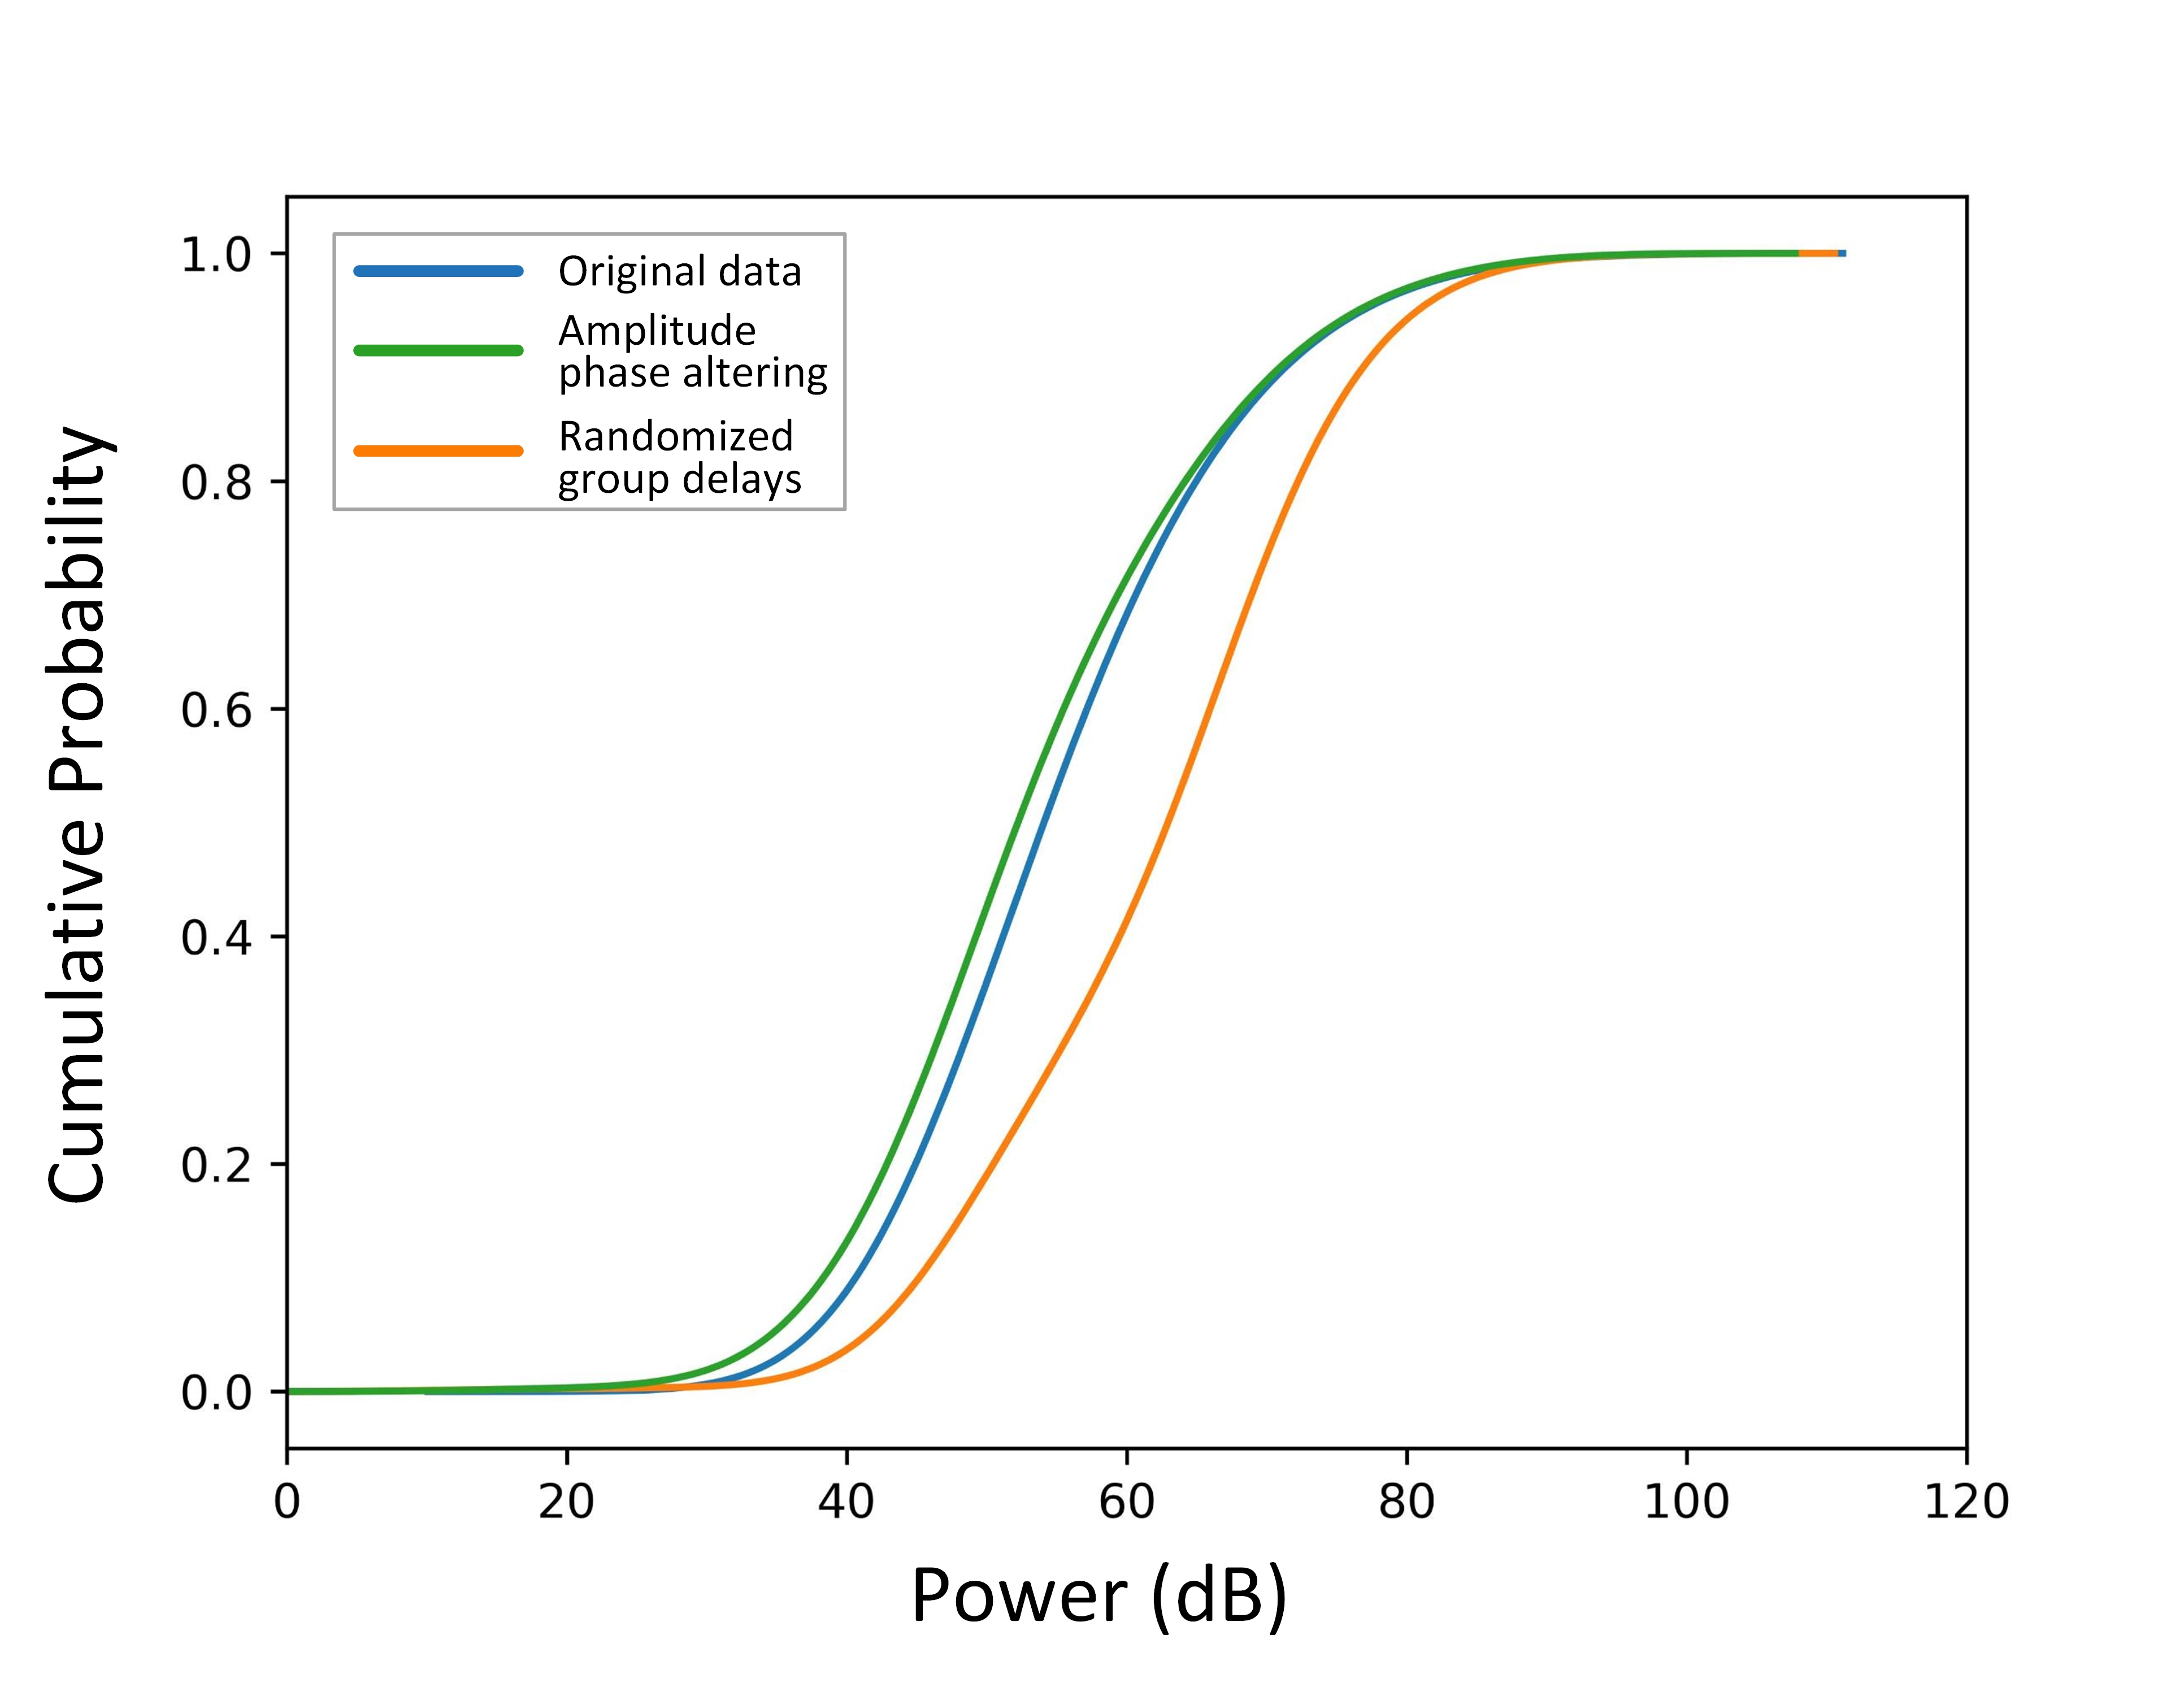
\includegraphics[width=0.6\textwidth]{Documents/cp.jpg}
    \caption{xxx.}
    \label{tab:CP}

\end{figure}

\subsection{Learning models}
In order to assess the effectiveness of the synthetic data approach, we examined the performance metrics of four distinct machine learning models: a basic two-layer Convolutional Neural Network (CNN), EfficientNetB0, VGG-16, and DeepConvNet. The simple CNN model comprising two CNN layers, followed by a max-pooling layer and a fully connected layer, was utilized as a baseline model. Additionally, we implemented both shallow and deep pre-trained CNN models by freezing the convolutional blocks and appending new fully connected layers.

\par The VGG-16 architecture has been widely adopted and recognized as a seminal work for its remarkable performance in image classification tasks \cite{simonyan2014very}. It comprises 16 weight layers, including 13 convolutional layers and three fully connected layers. We froze the convolutional layers and retrained three fully connected layers with 1024, 256, and 64 neurons and a dropout rate of 20\%. EfficientNetB0 comprises a series of inverted residual blocks, each followed by batch normalization and a Swish activation function \cite{tan2019efficientnet}. The architecture incorporates a depthwise separable convolution, which significantly reduces the number of parameters and computational costs compared to traditional convolutional layers. To adapt this model, we introduced two fully connected layers with 256 and 64 neurons, respectively, at the end of the architecture.


\section{Results}
CNN
CNN-LSTM
DeepConv
Efficientnet
NASNetMobile
MobileNetV2
VGG16
inceptiontime



\begin{table}[]
\begin{tabular}{|l|l|l|l|l|l|l|l|l|l|l|}
\hline
\multicolumn{1}{|c|}{\multirow{2}{*}{Models}} & \multicolumn{5}{c|}{Row data} & \multicolumn{5}{c|}{Synthetic data} \\ \cline{2-11} 
\multicolumn{1}{|c|}{}                        & AUC  & Accu  & F1 & Sen & Spe & AUC   & Accu   & F1   & Sen  & Spe  \\ \hline
CNN                                           &      &       &    &     &     &       &        &      &      &      \\ \hline
EfficientNetB0                                &      &       &    &     &     &       &        &      &      &      \\ \hline
VGG-16                                        &      &       &    &     &     &       &        &      &      &      \\ \hline
DeepConvNet                                   &      &       &    &     &     &       &        &      &      &      \\ \hline
\end{tabular}
\end{table}

\section{Discussion}
% The traditional approach to diagnosing heart murmurs involves auscultation, wherein physicians rely on their auditory skills and clinical experience to identify and interpret abnormal heart sounds. However, this method is subjective and susceptible to variability, leading to potential inaccuracies in diagnosis. Consequently, researchers have sought to develop more objective, reliable, and accurate tools for the assessment of heart murmurs, including advanced imaging techniques, such as echocardiography and cardiac magnetic resonance imaging (MRI), as well as machine learning algorithms and artificial intelligence applications.

%considering real-world situations for the model
%one reason that ML models are not good in the real-world scenario
\section{Conclusion}


\bibliographystyle{ieeetr}
\bibliography{ref}

\end{document}
